\section{Statystyki}

Przykładowe wykresy przedstawiające ilość zdobytej wiedzy wraz z upływem czasu (iteracji).
\nopagebreak

\begin{figure}[H]
	\centering
	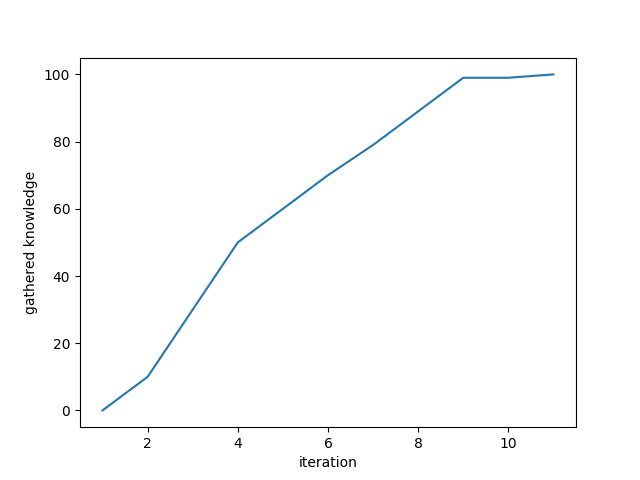
\includegraphics[width=130mm]{wykresy/learning_map-50x50_graph-2-50_res-10-100_p-1.png}
	\caption{Wykres dla mapy 20x20, 2 kliki, 100 agentów, 10 zasobów o wartości 100}
\end{figure}

\begin{figure}[H]
	\centering
	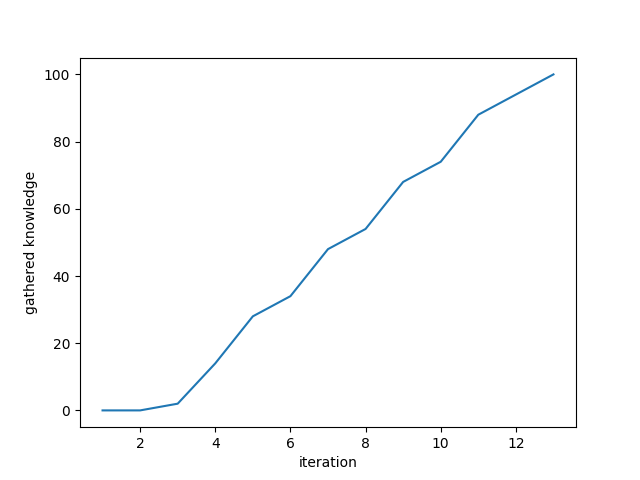
\includegraphics[width=130mm]{wykresy/learning_map-50x50_graph-20-5_res-10-100_p-1.png}
	\caption{Wykres dla mapy 20x20, 20 klikek, 100 agentów, 10 zasobów o wartości 100}
\end{figure}

Poniższe wykresy przedstawiają szybkość zdobywania wiedzy przez populację (ilośc iteracji potrzebnej do zebrania całej dostępnej wiedzy) w zależnośći ilości klik.
\nopagebreak

\begin{figure}[H]
	\centering
	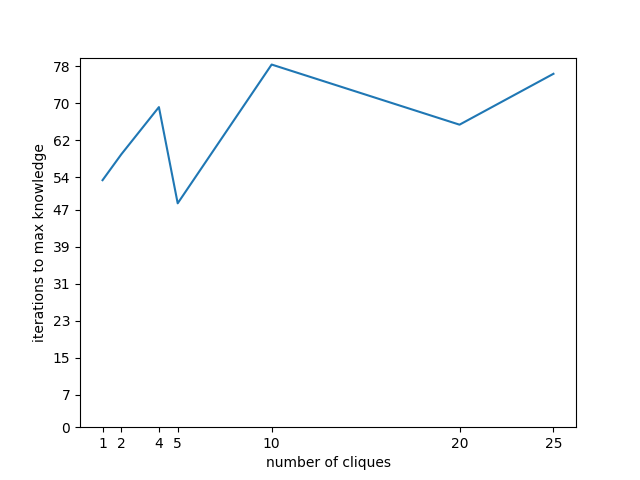
\includegraphics[width=130mm]{wykresy/different_number_of_cliques_map-20x20_graph-10-10_res-10-10_p-1.png}
	\caption{Wykres dla mapy 20x20, 100 agentów, 10 zasobów o wartości 10}
\end{figure}

Poniższe wykresy przedstawiają szybkość zdobywania wiedzy przez populację (ilośc iteracji potrzebnej do zebrania całej dostępnej wiedzy) w zależnośći od zasobów dostępnych na mapie.
\nopagebreak

\begin{figure}[H]
	\centering
	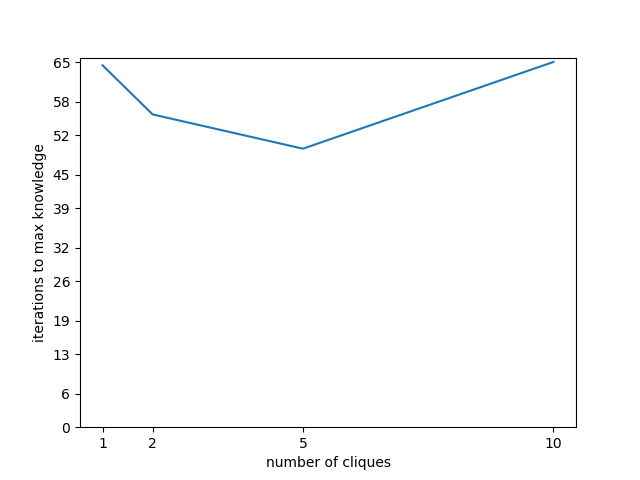
\includegraphics[width=130mm]{wykresy/different_number_of_cliques_map-20x20_graph-1-100_res-10-10_p-1.png}
	\caption{Wykres dla mapy 20x20, 1 kliki, 100 agentów, 10 zasobów o wartości 10}
\end{figure}

\begin{figure}[H]
	\centering
	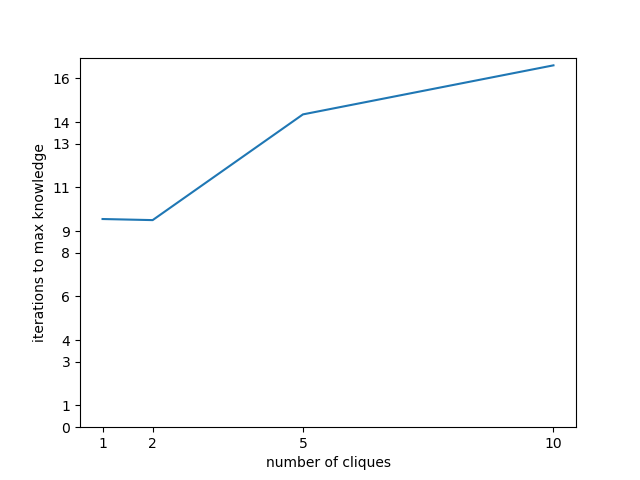
\includegraphics[width=130mm]{wykresy/different_number_of_cliques_map-20x20_graph-1-100_res-2-50_p-1.png}
	\caption{Wykres dla mapy 20x20, 1 kliki, 100 agentów, 2 zasobów o wartości 50}
\end{figure}

\begin{figure}[H]
	\centering
	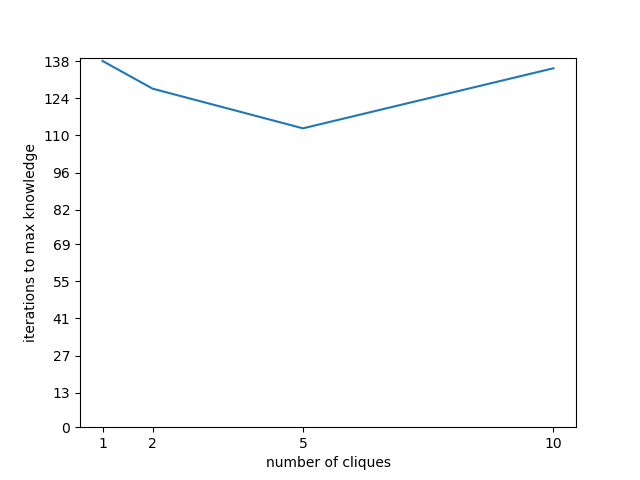
\includegraphics[width=130mm]{wykresy/different_number_of_cliques_map-20x20_graph-1-100_res-20-5_p-1.png}
	\caption{Wykres dla mapy 20x20, 1 kliki, 100 agentów, 20 zasobów o wartości 5}
\end{figure}

\begin{figure}[H]
	\centering
	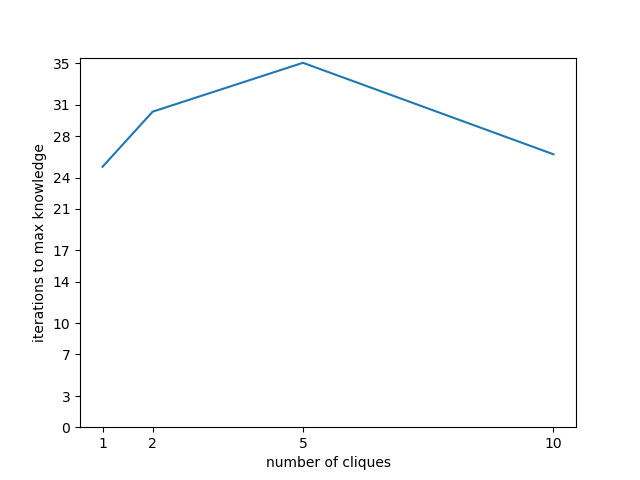
\includegraphics[width=130mm]{wykresy/different_number_of_cliques_map-20x20_graph-1-100_res-5-20_p-1.png}
	\caption{Wykres dla mapy 20x20, 1 kliki, 100 agentów, 5 zasobów o wartości 20}
\end{figure}

Wykres przedstawia zależność szybkości zdobywanej wiedzy od parametry p - prawdopodobieństwa przekazania wiedzy.
\nopagebreak

\begin{figure}[H]
	\centering
	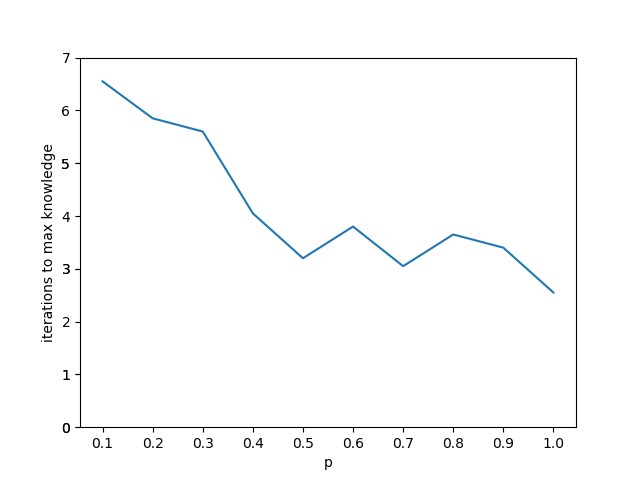
\includegraphics[width=130mm]{wykresy/different_p_map-30x30_graph-1-125_res-50-23_p-1.png}
	\caption{Wykres dla mapy 30x30, 1 kliki, 125 agentów, 50 zasobów o wartości 23}
\end{figure}

